%The next six (6) lines are here because we only have on appendix. This removes the trailing label "A" which is unecessary since there is only one appendix for the TOC entry. Added by Sarah July 23, 2026
\makeatletter
\renewcommand{\thechapter}{A} 
\setcounter{chapter}{1} 
\renewcommand{\chaptername}{Appendix} 
\renewcommand{\thechapter}{} 
\makeatother

\chapter{Naming Convention for Diamond Samples}
\label{SampleTracking}

%The next four (4) lines allows reinstitutes the trailing "A" now that the title of the chapter has printed. It allows for tables and figures to be labeled A.1, A.2, etc. Added by Sarah July, 23, 2026
\renewcommand{\thechapter}{A}
\setcounter{figure}{0}
\setcounter{table}{0}
\makeatother

\indent

The first step in characterizing diamond samples is naming the sample. As samples go through several changes, sample names need to be informative and modifiable such that origination and process history is preserved. A three part naming convention was developed. The naming convention starts with a source code which indicates the supplier or growth reactor, see Figure \ref{fig:nameSource}. The second part of the naming convention is the acquisition code which indicates the year the sample was acquired and the sequential order the sample was received within that year, see Figure \ref{fig:nameAcq}. The last part of the naming convention is the modification code which add or increments an alphabetical character for processing that modifies the bulk material properties. The modification code for surface treatments is a numeric character that should be added or incremented for subsequent surface treatments, see Figure \ref{fig:nameMod}. A graphical example of the implementation of this naming convention is show in Figure \ref{fig:nameEx}.

\begin{figure}
    \centering
    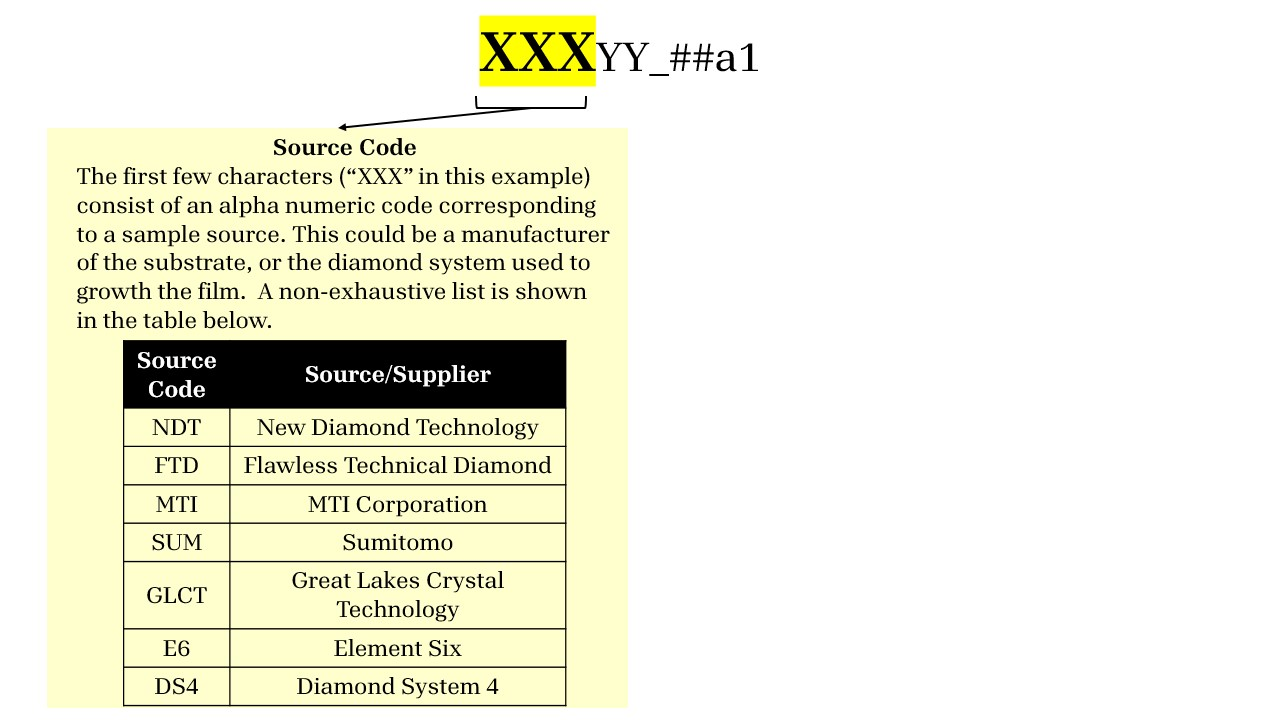
\includegraphics[width=1\linewidth]{figures/Slide2.jpg}
    \caption{Source code description for sample naming convention.}
    \label{fig:nameSource}
\end{figure}

\begin{figure}
    \centering
    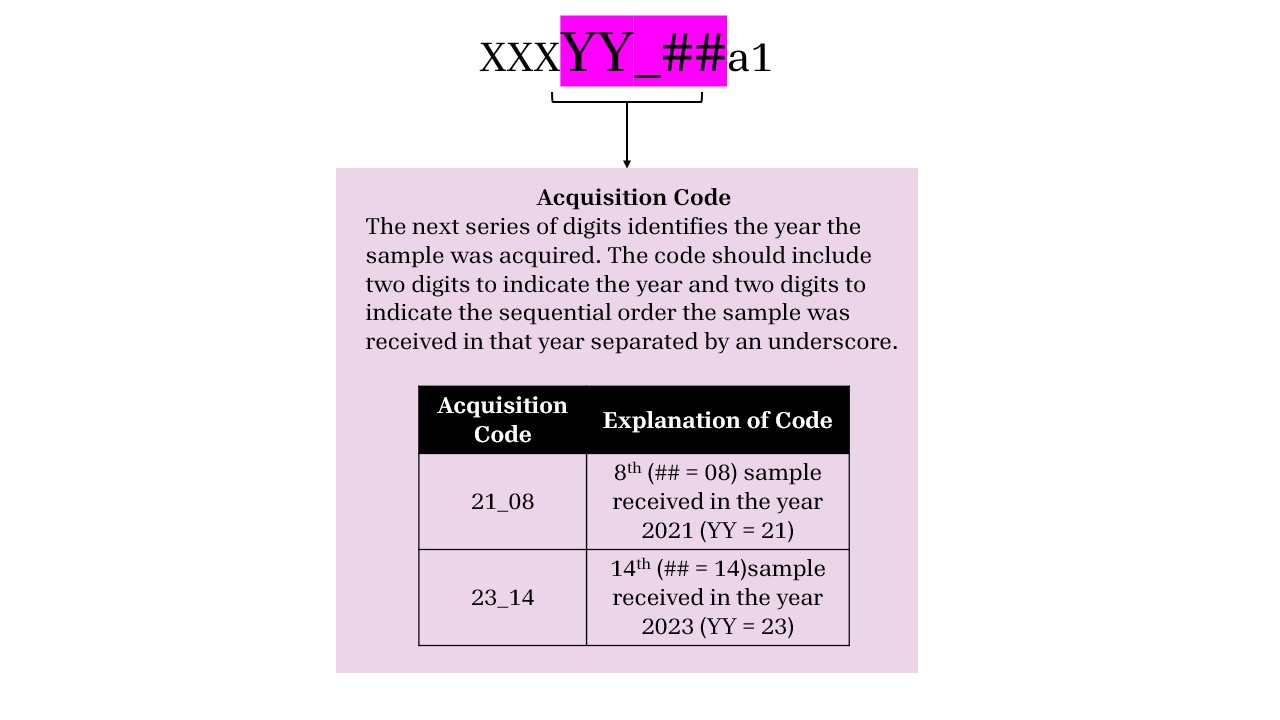
\includegraphics[width=1\linewidth]{figures/Slide3.jpg}
    \caption{Acquisition code description for sample naming convention.}
    \label{fig:nameAcq}
\end{figure}

\begin{figure}
    \centering
    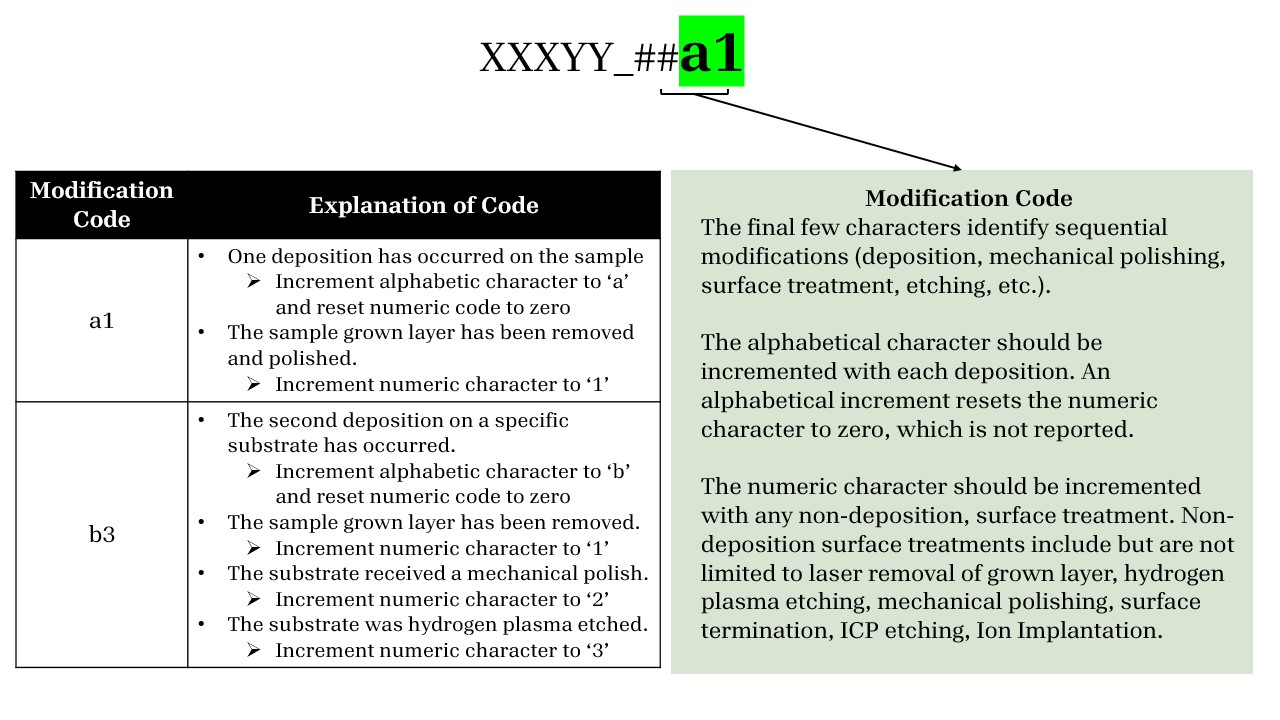
\includegraphics[width=1\linewidth]{figures/Slide4.jpg}
    \caption{Modification code description for sample naming convention.}
    \label{fig:nameMod}
\end{figure}

\begin{figure}
    \centering
    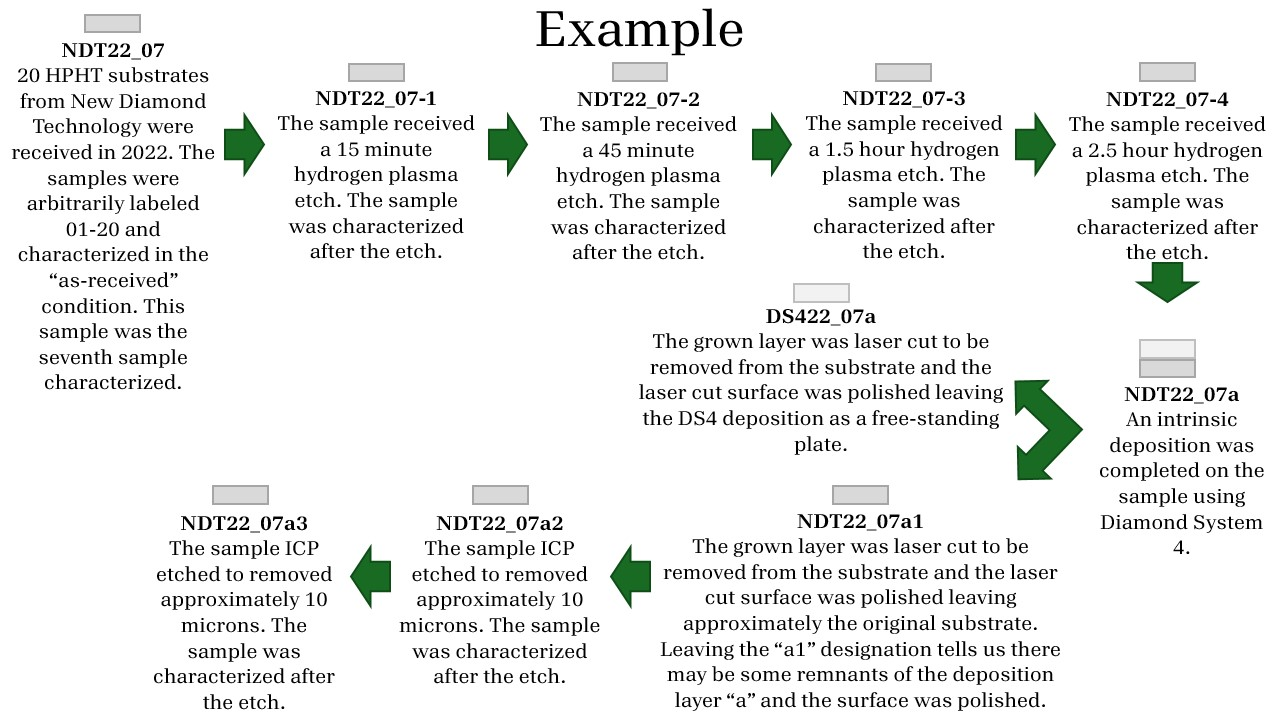
\includegraphics[width=1\linewidth]{figures/Slide6.jpg}
    \caption{Graphical example of naming convention implementation.}
    \label{fig:nameEx}
\end{figure}
